\section{Methods for Learning from SITS Data}

\begin{frame}{Complete Training Pipeline Overview}
    \renewcommand{\currprop}{0.6\textheight}
    
    \begin{block}{Pretraining, Finetuning and Error Rebuttal}
        \only<1| handout:0>{During the training stage, we first retrieve the unlabeled SITS samples.}%
        \only<2| handout:0>{Samples have already been downloaded in the previous flow using our library.}%
        \only<3| handout:0>{These samples undergo data augmentation to self-supervisedly pre-train the model using SSL strategies.}%
        \only<4| handout:0>{The pre-trained backbone is then fine-tuned using a smaller, curated set of labeled samples.}%
        \only<5| handout:0>{Using these fine-tuned embeddings, we train a distinct Gaussian Mixture Model (GMM) per class for the ORDER anomaly detection framework.}%
        \only<6| handout:0>{In the inference stage, the standalone classifier makes an initial class prediction based on the time series.}%
        \only<7| handout:1>{ORDER GMM pipeline verifies the prediction, acting as a critical gatekeeper to confirm or reject the classifier's output.}%
    \end{block}
	\begin{figure}
		\centering
		\includegraphics<1| handout:0>[height=\currprop]{figures_slides/meth_graphical_abstract-6.pdf}%
		\includegraphics<2| handout:0>[height=\currprop]{figures_slides/meth_graphical_abstract-6-marked.jpg}%
		\includegraphics<3| handout:0>[height=\currprop]{figures_slides/meth_graphical_abstract-5.pdf}%
		\includegraphics<4| handout:0>[height=\currprop]{figures_slides/meth_graphical_abstract-4.pdf}%
		\includegraphics<5| handout:0>[height=\currprop]{figures_slides/meth_graphical_abstract-3.pdf}%
		\includegraphics<6| handout:0>[height=\currprop]{figures_slides/meth_graphical_abstract-2.pdf}%
        \includegraphics<7| handout:1>[height=\currprop]{figures_slides/meth_graphical_abstract-1.pdf}%
	\end{figure}
\end{frame}

% --- SHALLOW MODELS ---

\begin{frame}{Methodology: Shallow Learning Baselines}
    \begin{block}{Feature Engineering for SITS}
        Unlike deep architectures, Shallow Learning algorithms cannot natively process time series of varying lengths. To establish a baseline, we reduced the temporal dimensionality by calculating \textbf{monthly averages}, resampling the SITS to 12 fixed time steps.
    \end{block}
    
    \pause
    
    \begin{block}{Evaluated Models}
        \begin{itemize}
            \item \textbf{Random Forest (RF) \& LightGBM:} Robust ensemble methods based on decision trees.
            \item \textbf{Support Vector Machine (SVM):} Classical maximum-margin classifier.
            \item \textbf{Multi-Layer Perceptron (MLP):} A standard feed-forward neural network.
        \end{itemize}
    \end{block}
\end{frame}

\begin{frame}{Deep Learning Architectures}
    \renewcommand{\currprop}{0.6\textheight}
    
    \begin{block}{Backbone construction}
        {Let's take a closer look at the architectures of Deep Learning models.}%
    \end{block}
	\begin{figure}
		\centering
		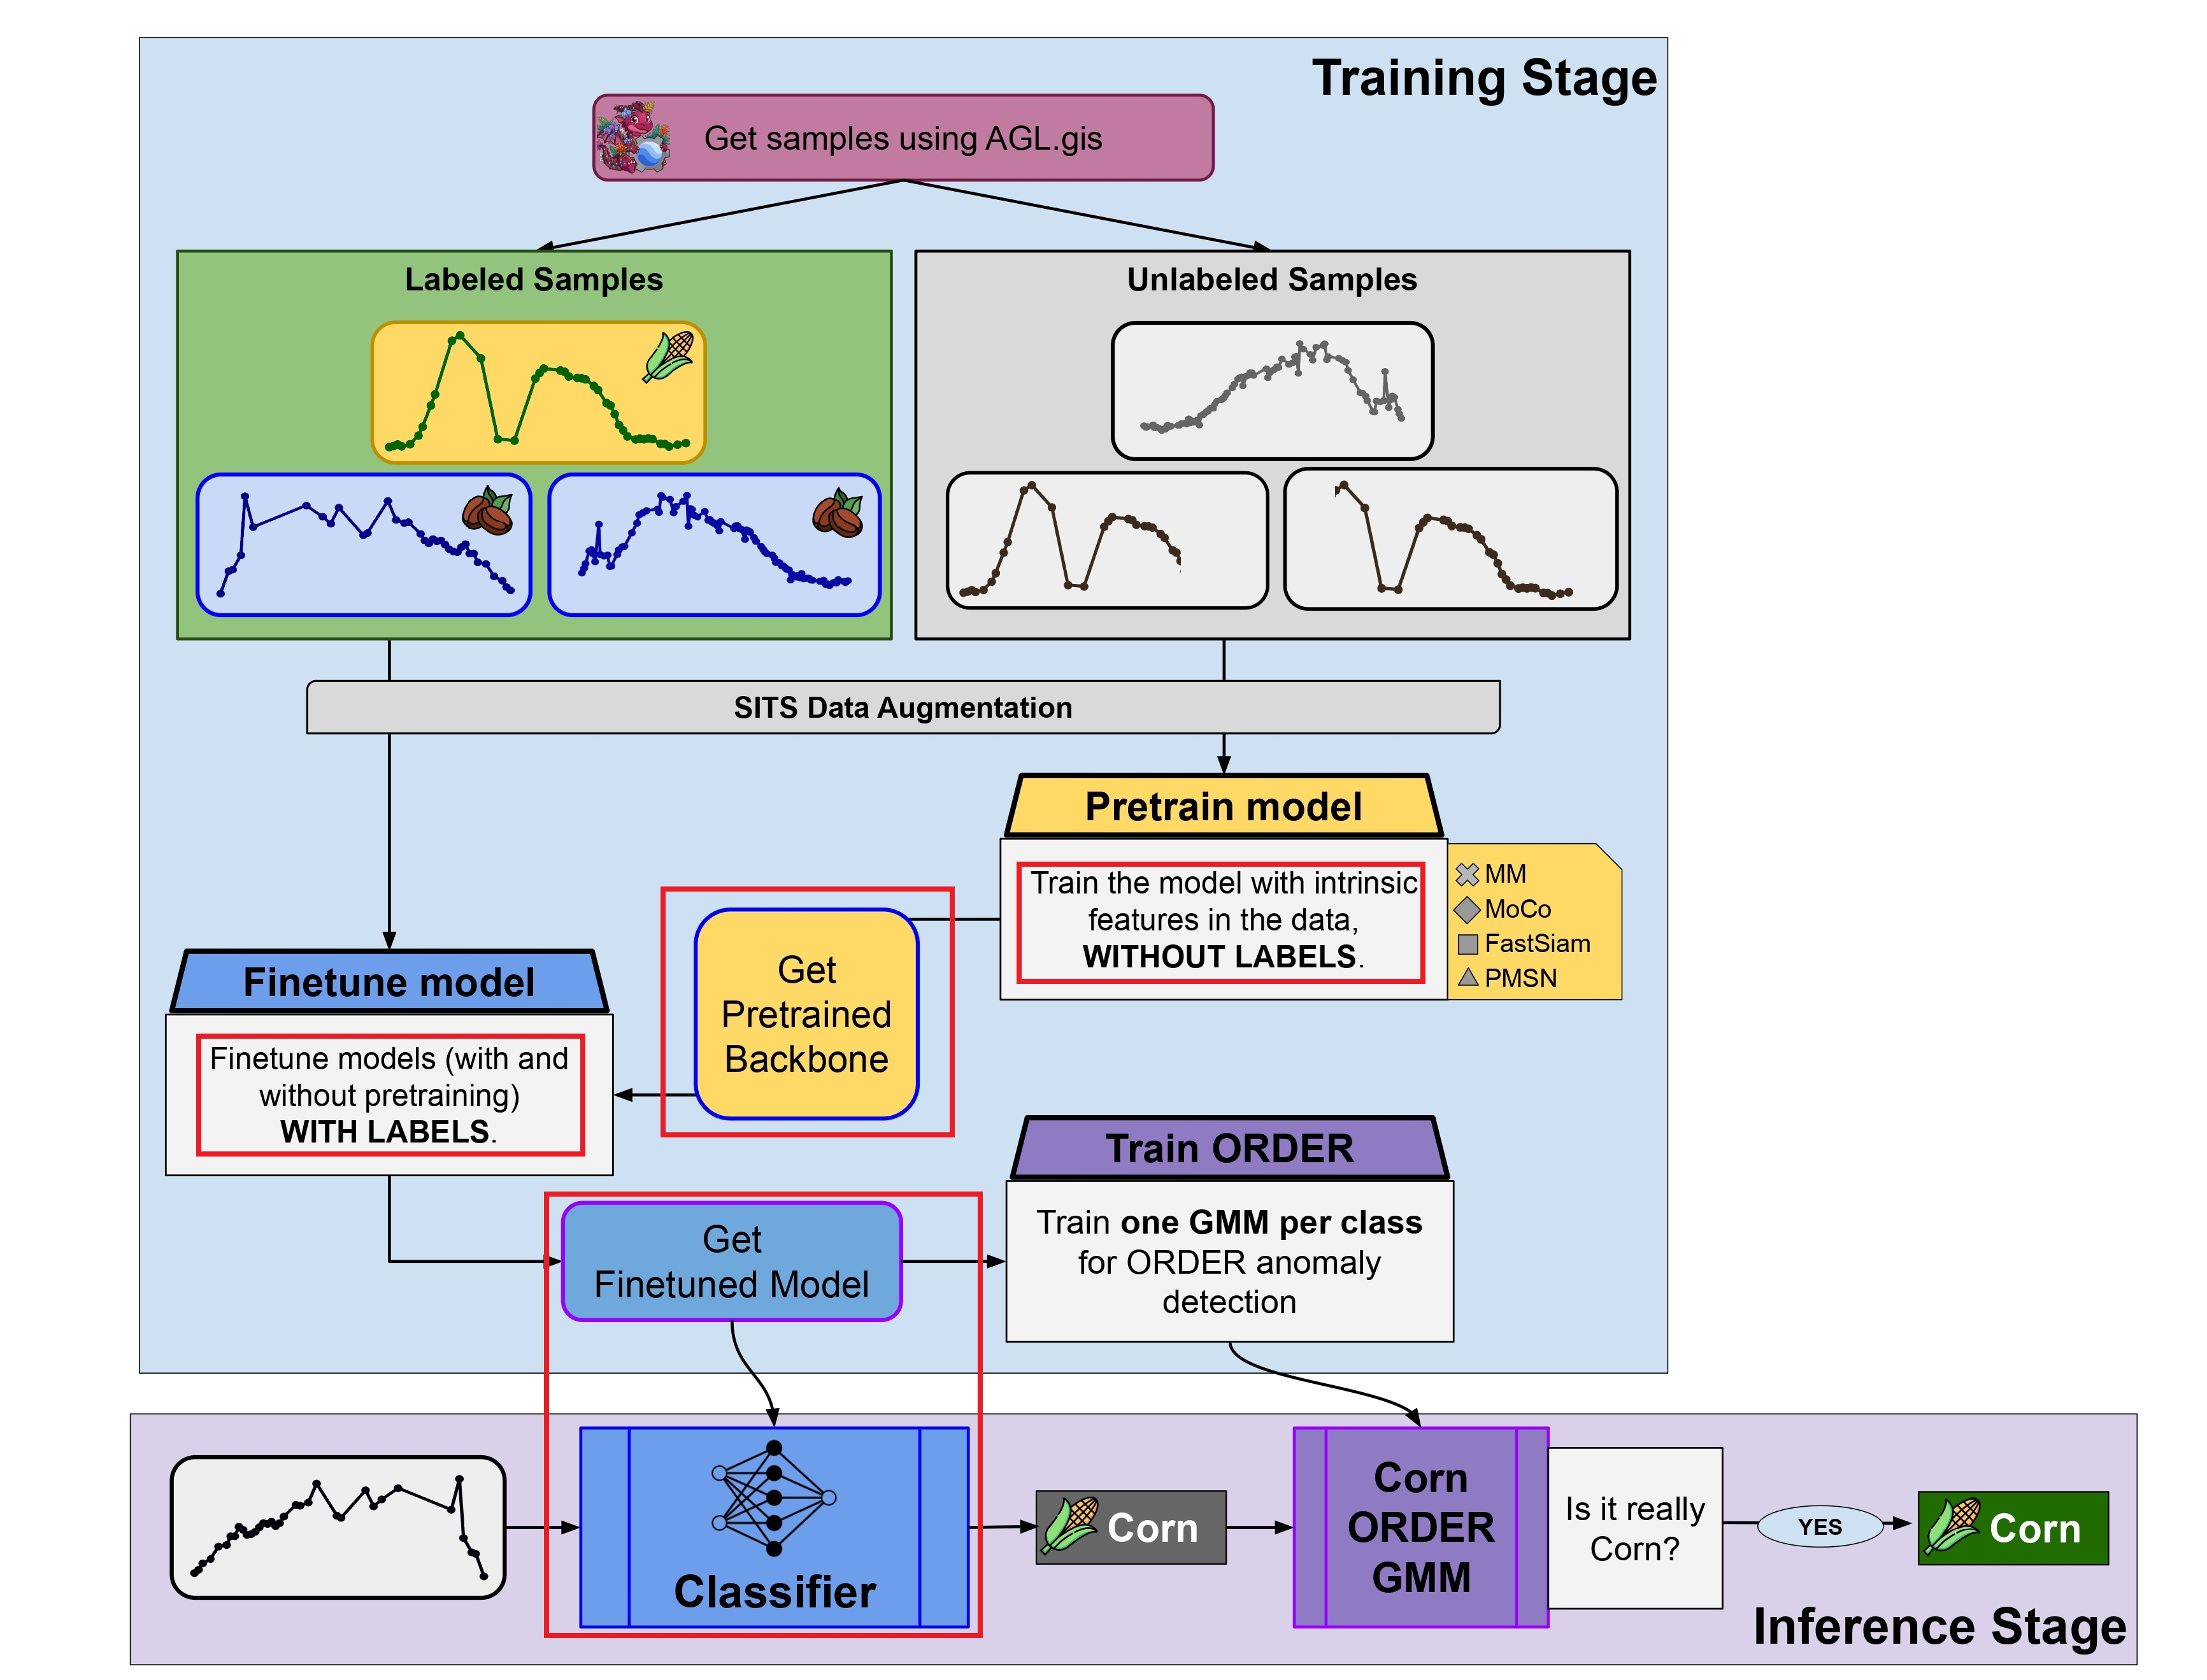
\includegraphics[height=\currprop]{figures_slides/meth_graphical_abstract_models.jpg}%
	\end{figure}
\end{frame}

\begin{frame}{Deep Learning Architectures}    
    \begin{enumerate}
        \item \textbf{SITS-CNN (ConvNeXt-based):} Adapts modern 2D vision techniques to 1D sequences, utilizing large convolutional kernels (size 7) to efficiently capture broad temporal contexts. \textbf{(Ours)}
        \item \textbf{SITS-LSTM (Recurrent):} Employs Bidirectional GRUs with early Day-of-the-Year (DoY) positional encoding, capturing forward and backward temporal dependencies for fair baseline comparisons. \textbf{(Ours)}
        \item \textbf{SITS-BERT (Transformer):} Uses standard self-attention (3 layers, 8 heads) to process the entire sequence simultaneously, fusing inputs with DoY encodings to preserve agricultural calendars. \footnote[1]{\url{https://ieeexplore.ieee.org/document/9252123}}
    \end{enumerate}
\end{frame}

\begin{frame}{Deep Learning Architectures}    
    \begin{enumerate}
        \item \textbf{SITS-BERT++ (Enhanced Transformer):} An architectural evolution of SITS-BERT featuring increased capacity (12 heads) and a dual activation strategy (Swish/GeLU) for optimized gradient flow. \footnote[1]{\url{https://ieeexplore.ieee.org/document/10899708}}
        \item \textbf{SITS-Mamba (State Space Model):} A lightweight, post-Transformer approach using Selective State Spaces (S6) to filter irrelevant data, offering high-level reasoning with linear $\mathcal{O}(L)$ efficiency. \textbf{(Ours)}
    \end{enumerate}
\end{frame}

\begin{frame}{SSL Pretrain}
    \renewcommand{\currprop}{0.6\textheight}
    
    \begin{block}{Better than random weights}
        {Let's take a closer look how SSL pretraining works in the pipeline.}%
    \end{block}
	\begin{figure}
		\centering
		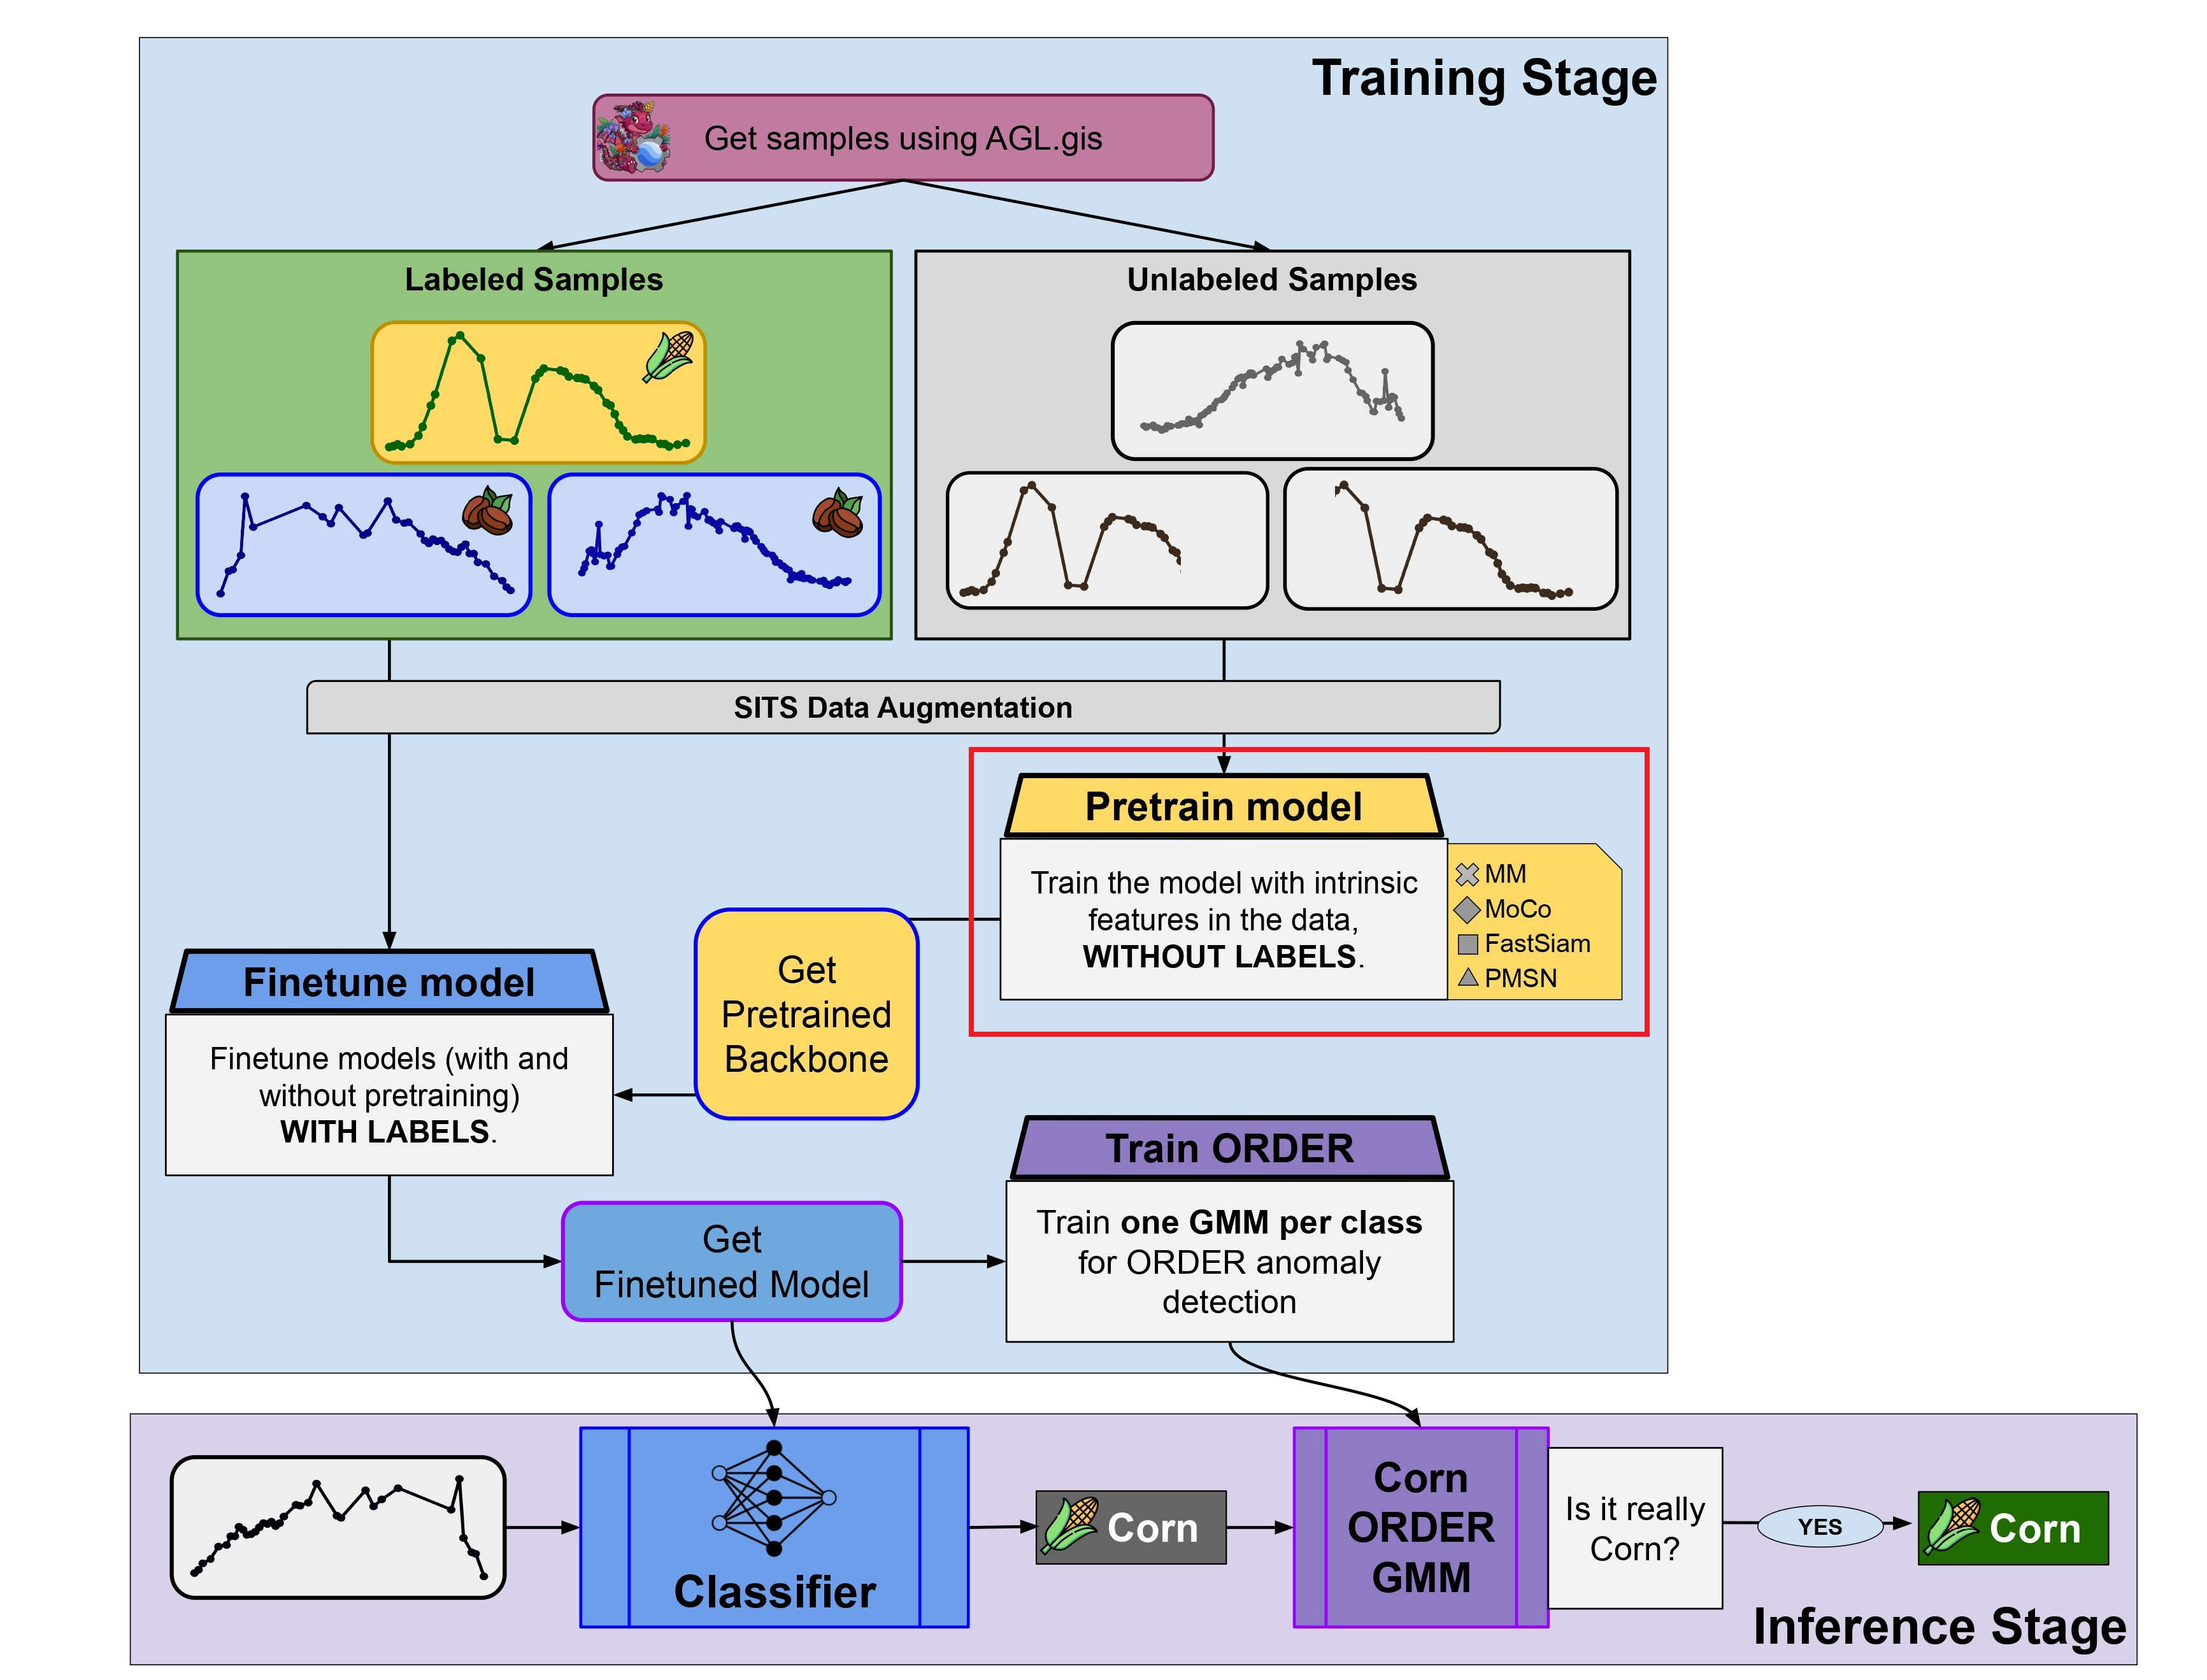
\includegraphics[height=\currprop]{figures_slides/meth_graphical_abstract_ssl.jpg}%
	\end{figure}
\end{frame}

\begin{frame}{SSL Pretrain}
    \renewcommand{\currprop}{0.5\textheight}
    
    \begin{block}{Deep Feature Extraction from Pretrained Networks}
        \only<1| handout:0>{The self-supervised learning process begins with an original, unlabeled SITS sample.}%
        \only<2| handout:0>{Data augmentation techniques generate distinct altered views of this same original sequence.}%
        \only<3| handout:0>{Driven by the FastSiam architecture, the model forces these augmented views closer together in the pre-training embedding space.}%
        \only<4| handout:0>{Simultaneously, a database of negative samples provides distinct, unrelated time series for contrastive learning.}%
        \only<5| handout:0>{Applying the MoCo paradigm, the model actively pushes these negative embeddings far away from the positive anchor.}%
        \only<6| handout:0>{A Masked Modeling (MM) approach further challenges the network by dropping random temporal segments from the signal.}%
        \only<7| handout:0>{The network learns intrinsic structural patterns by attempting to accurately reconstruct these masked segments.}%
        \only<8| handout:1>{Ultimately, the PMSN strategy unifies these tasks—pulling similar views, pushing negative samples, and reconstructing masks—into a single, pre-training mechanism.}%
    \end{block}
	\begin{figure}
		\centering
		\includegraphics<1| handout:0>[height=\currprop]{figures_slides/meth_ssl-7.pdf}%
		\includegraphics<2| handout:0>[height=\currprop]{figures_slides/meth_ssl-6.pdf}%
        \includegraphics<3| handout:0>[height=\currprop]{figures_slides/meth_ssl-5.pdf}%
        \includegraphics<4| handout:0>[height=\currprop]{figures_slides/meth_ssl-4.pdf}%
        \includegraphics<5| handout:0>[height=\currprop]{figures_slides/meth_ssl-3.pdf}%
        \includegraphics<6| handout:0>[height=\currprop]{figures_slides/meth_ssl-2.pdf}%
        \includegraphics<7| handout:0>[height=\currprop]{figures_slides/meth_ssl-1.pdf}%
        \includegraphics<8| handout:1>[height=\currprop]{figures_slides/meth_ssl.pdf}%
	\end{figure}
\end{frame}

\begin{frame}{ORDER - In details}
    \renewcommand{\currprop}{0.6\textheight}
    
    \begin{block}{The Last Step}
        {Let's take a closer look how ORDER anomaly detection works in the pipeline.}%
    \end{block}
	\begin{figure}
		\centering
		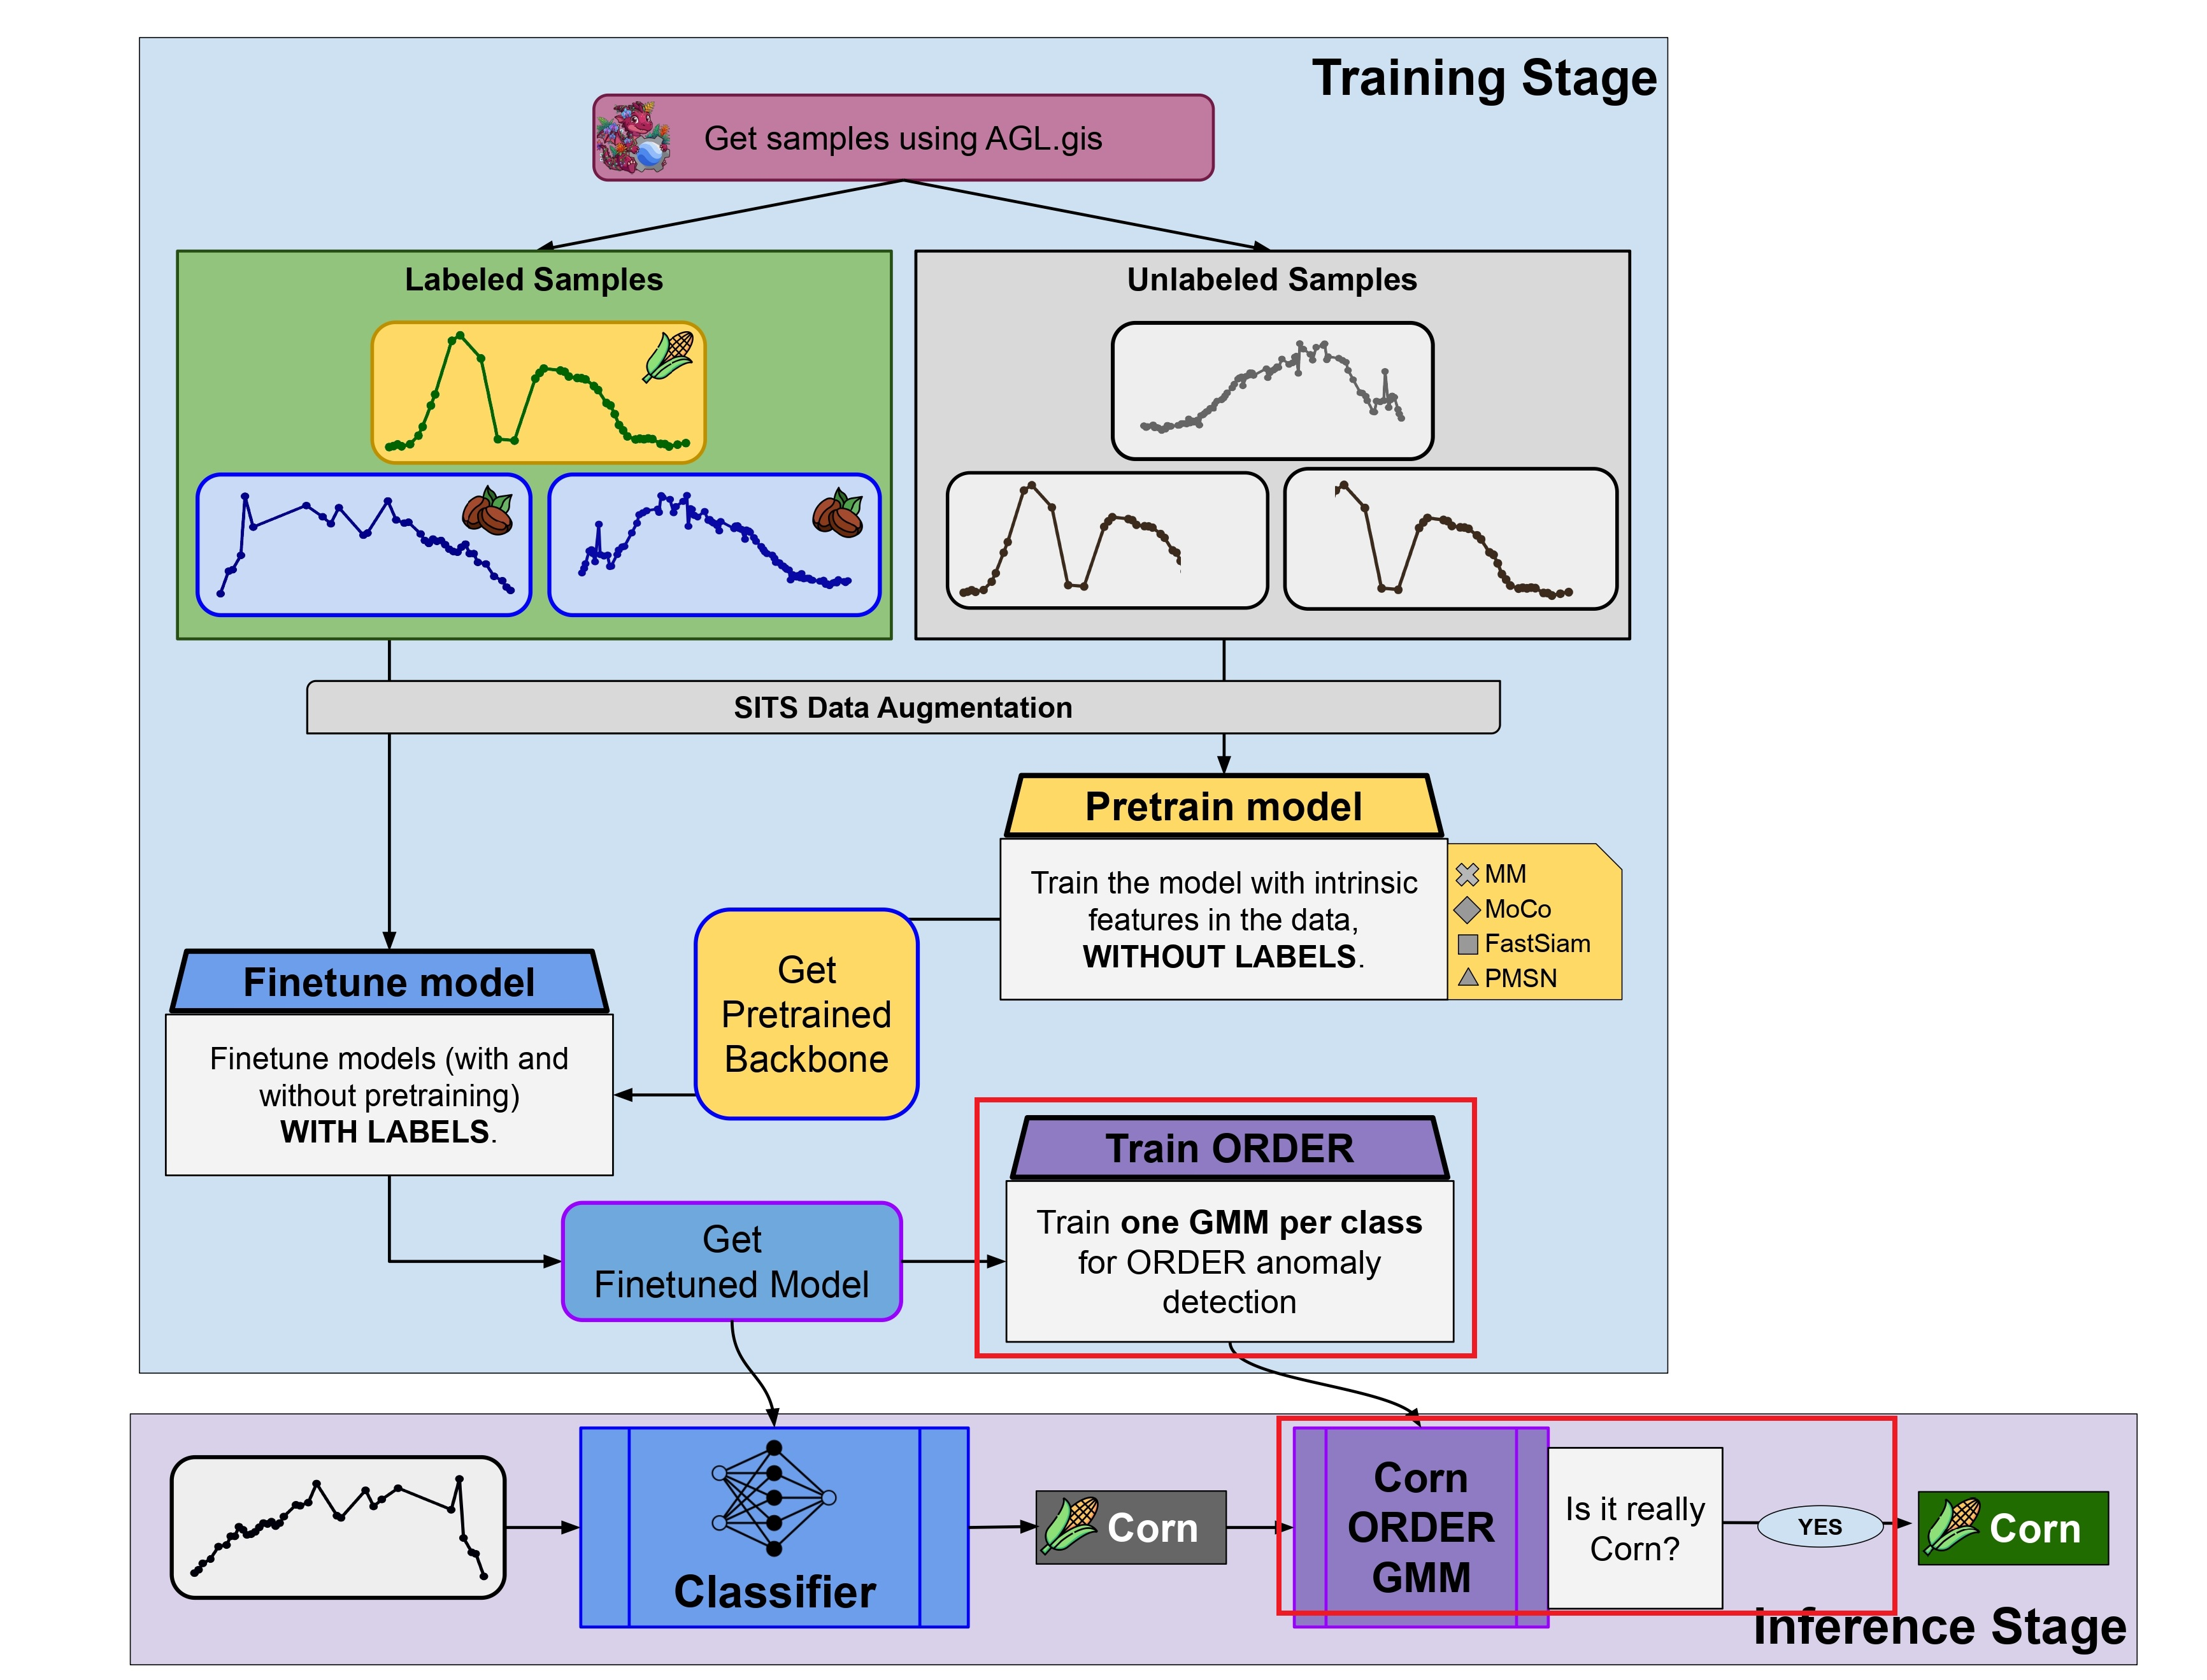
\includegraphics[height=\currprop]{figures_slides/meth_graphical_abstract_order.jpg}%
	\end{figure}
\end{frame}

\begin{frame}{ORDER - In details}
    \renewcommand{\currprop}{0.5\textheight}
    
    \begin{block}{Open-set Recognition for Discriminative Error Rebutta}
        \only<1| handout:0>{The system utilizes the trainig and validation dataset to pass representations through the fine-tuned model backbone.}%
        \only<2| handout:0>{Within the embedding space, the training samples initialize one distinct GMM for each crop class.}%
        \only<3| handout:0>{Both positive and negative validation samples are subsequently mapped to evaluate these class boundaries.}%
        \only<4| handout:0>{The hyperparameter optimization loop begins by scoring all validation sets against the fitted GMMs.}%
        \only<5| handout:0>{This process actively maximizes the spatial separation between clean predictions and hard, out-of-distribution samples.}%
        \only<6| handout:0>{A dynamic confidence threshold is statistically determined for each class by maximizing the F1-score.}%
        \only<7| handout:0>{To ensure ultimate reliability, a conservative fallback mechanism (GEMOS) is integrated for cases with very few correct or incorrect validation samples.}%
        \only<8| handout:0>{During class fixation, the system evaluates: 'Is the GMM score greater than the dynamic threshold?'}%
        \only<9| handout:0>{At inference time, unseen time-series samples are projected into the classifier embedding space, as usual.}%
        \only<10| handout:0>{The fine-tuned classification head assigns a preliminary label to the new inference sample.}%
        \only<11| handout:1>{If the score exceeds the threshold, the prediction is trusted; otherwise, the sample is safely flagged as Unknown.}%
    \end{block}
	\begin{figure}
		\centering
		\includegraphics<1| handout:0>[height=\currprop]{figures_slides/meth_models-10.pdf}%
		\includegraphics<2| handout:0>[height=\currprop]{figures_slides/meth_models-9.pdf}%
		\includegraphics<3| handout:0>[height=\currprop]{figures_slides/meth_models-8.pdf}%
		\includegraphics<4| handout:0>[height=\currprop]{figures_slides/meth_models-7.pdf}%
		\includegraphics<5| handout:0>[height=\currprop]{figures_slides/meth_models-6.pdf}%
        \includegraphics<6| handout:0>[height=\currprop]{figures_slides/meth_models-5.pdf}%
        \includegraphics<7| handout:0>[height=\currprop]{figures_slides/meth_models-4.pdf}%
        \includegraphics<8| handout:0>[height=\currprop]{figures_slides/meth_models-3.pdf}%
        \includegraphics<9| handout:0>[height=\currprop]{figures_slides/meth_models-2.pdf}%
        \includegraphics<10| handout:0>[height=\currprop]{figures_slides/meth_models-1.pdf}%
        \includegraphics<11| handout:1>[height=\currprop]{figures_slides/meth_models.pdf}%
	\end{figure}
\end{frame}